\chapter{Cohesive Subgroups: Illustration, Implementation and Accuracy}
\label{appendix_cohesive_groups}

\section{Illustration of the heuristics}
\label{illustration}

In order to illustrate how the proposed heuristics works, we will use a convenient synthetic network with 99 nodes and 200 edges where $\kappa \neq \delta$. This network is based on a two dimensional grid of 5 by 5 nodes. In each corner of the grid we attach a Petersen graph ($P$), linked by two edges to the grid. Thus the only four nodes of the grid with degree 2 are linked to a Petersen graph. All nodes of the grid are therefore part of a 3-core. Each $P$ is linked to two complete graphs with 5 nodes ($K_5$); in two cases those two $K_5$ overlap in only one node and in the other two cases, they overlap in two nodes. The Petersen graph is linked by three edges to one of the $K_5$, thus making one of each $K_5$ part of a tricomponent along with $P$. In the case of the two $K_5$ that overlap only on one node, the outer $K_5$ has also one edge linking one of its nodes with one node of $P$ nodes, in order to make the whole graph biconnected (see figure \ref{fig:example}). Petersen graphs have node connectivity 3 and complete graphs with 5 nodes have node connectivity 4. Notice that the whole example graph is biconnected and a 3-core, but it has three levels of node connectivity: 2 for the grid, 3 for the Petersen graphs ($P$) and 4 for the complete graphs of 5 nodes ($K_5$).


\begin{figure}[H]
\centering
%\subfloat[Nodes colored by core number. Notice that the 3-core includes all nodes in the graph.]{
%\label{fig:core}
%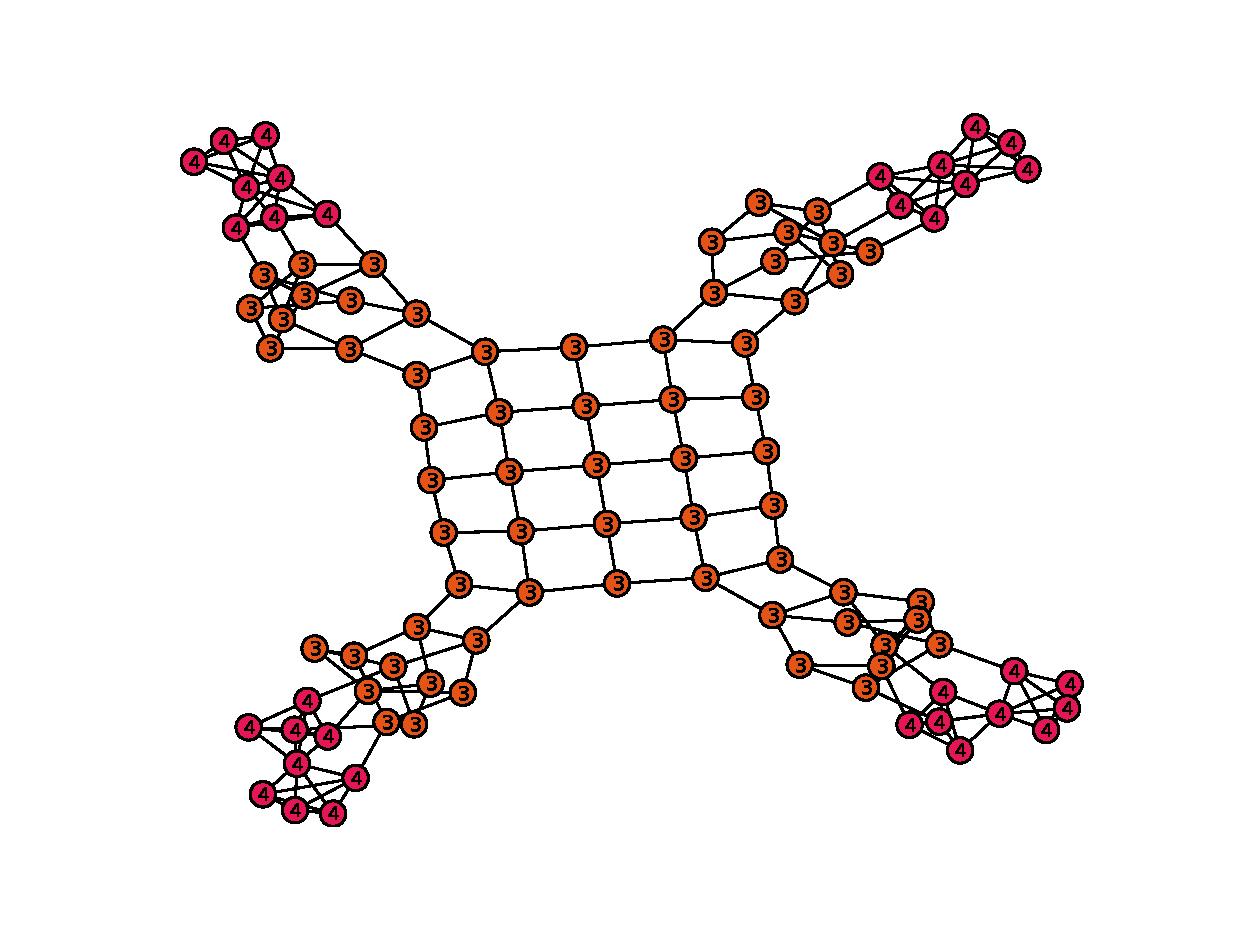
\includegraphics[scale=0.32]{figures/illustrative_core}
%}
%\hspace{.05in}
\subfloat[Nodes colored by component number according to our algorithm. Note the error when two $K_5$ overlap in two nodes]{
\label{fig:component}
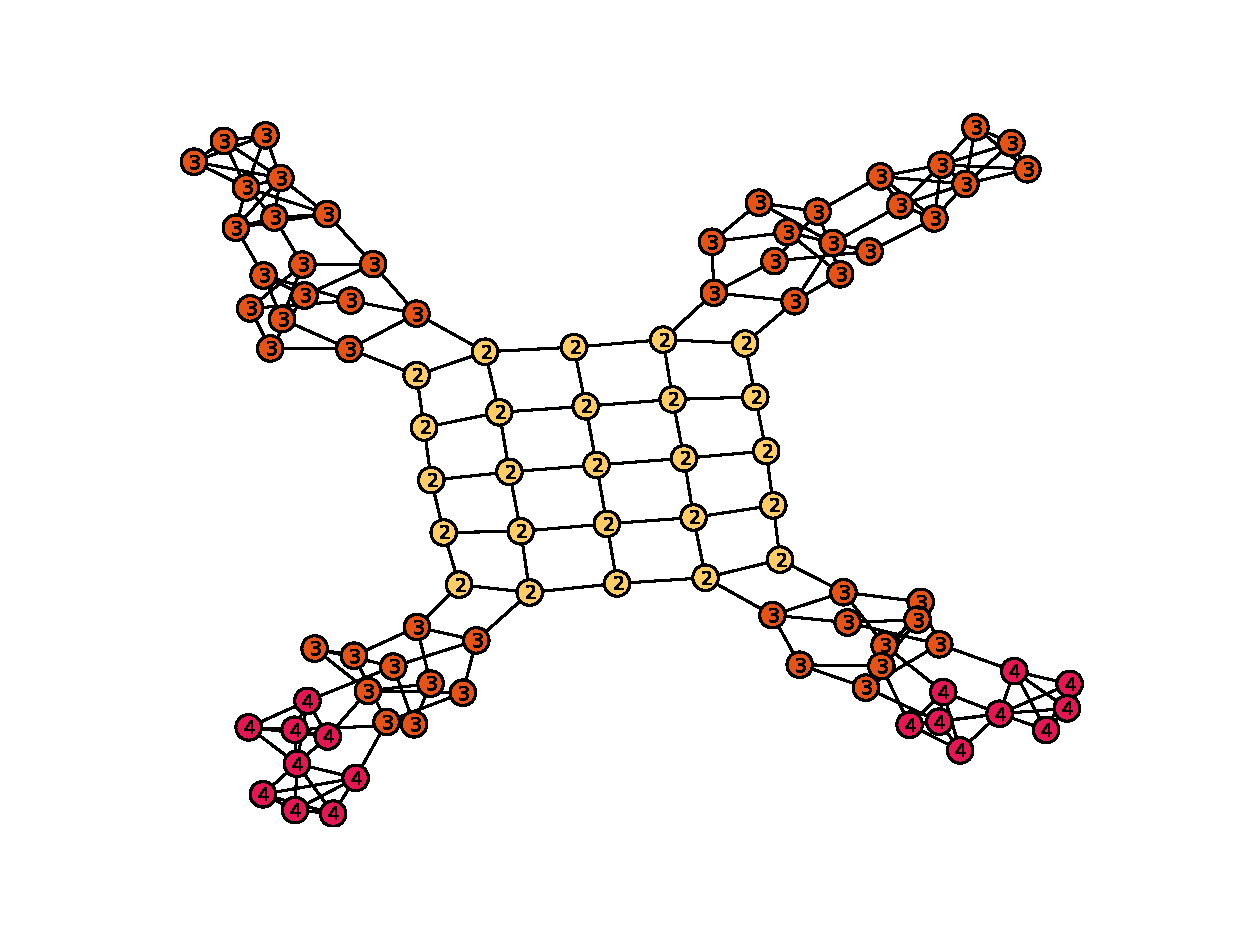
\includegraphics[scale=0.36]{figures/illustrative_knumber}
}
\hspace{.05in}
\subfloat[Nodes colored by component number according to Moody \& White algorithm.]{
\label{fig:component}
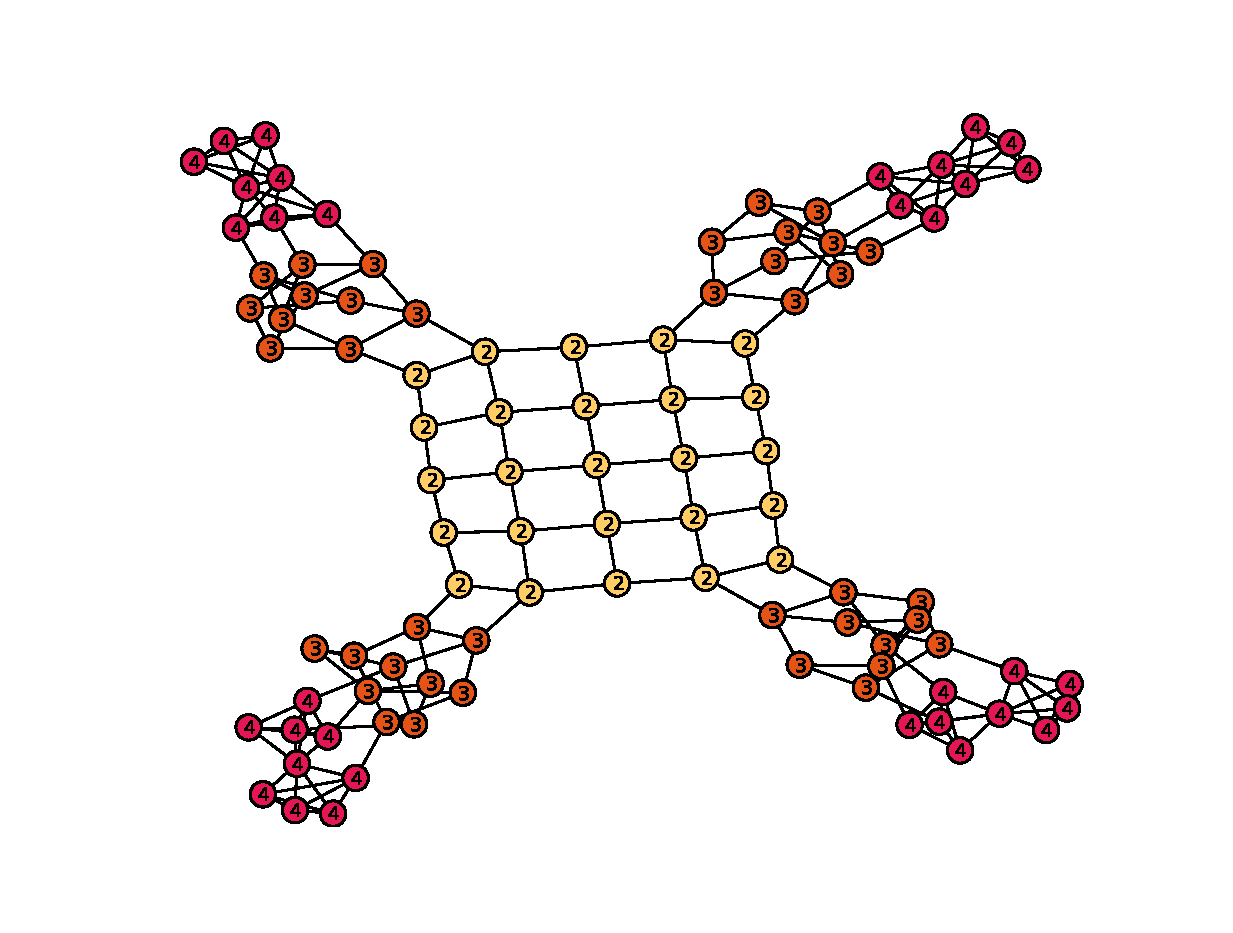
\includegraphics[scale=0.36]{figures/illustrative_knumber_exact}
}
\hspace{.05in}

\caption[Example synthetic graph for illustration.]{Synthetic graph composed of a two dimensional grid of 25 nodes, four Petersen graphs ($P$) with ten nodes each (with $\kappa = 3$) linked by two edges to the grid, and eight complete graphs $K_5$ (with $\kappa = 4$) linked by three edges to each Petersen graph. In two cases $K_5$ overlap in 1 node and in the other two cases they overlap in 2 nodes. The whole graph is biconnected and also a tricore. Notice that our algorithm fails to classify the two $K_5$ that overlap in two nodes as 4-components. See text and  figure figure  \ref{fig:example_4} for details.}
\label{fig:example}
\end{figure}

%\begin{landscape}

\begin{figure}[H]
\centering
\subfloat[Auxiliary graph $H$ for $k=3$ computed using White \& Newman's approximation algorithm for local node connectivity.]{
\label{fig:aux3}
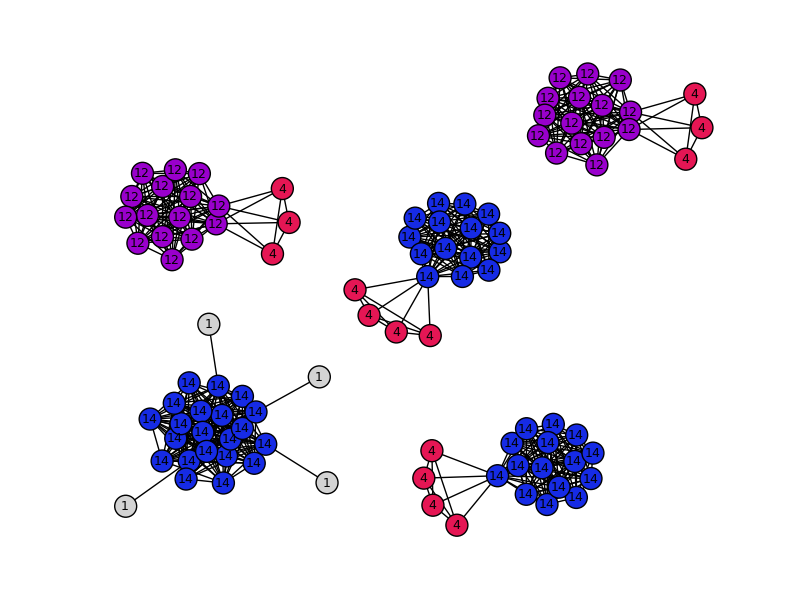
\includegraphics[scale=0.36]{figures/illustrative_aux_graph_3}
}
\hspace{.05in}
\subfloat[Auxiliary graph $H$ for $k=3$ computed using flow-based connectivity algorithm for local node connectivity.]{
\label{fig:aux3_ex}
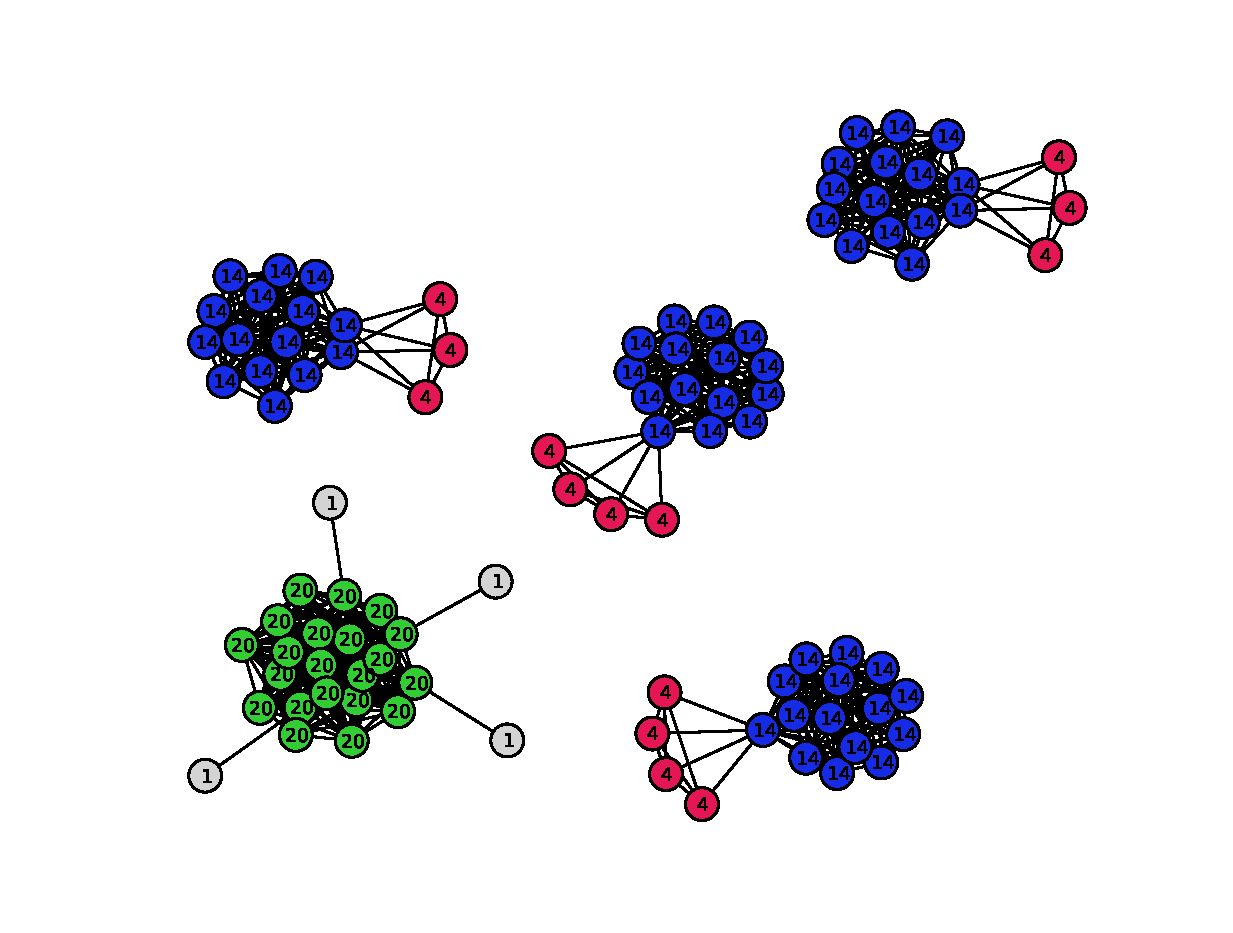
\includegraphics[scale=0.36]{figures/illustrative_aux_graph_3_exact}
}
\hspace{.05in}
\subfloat[All subgraphs $H_{candidate}$ from $H_3$ computed using White \& Newman's approximation algorithm for local node connectivity.]{
\label{fig:aux3_cand}
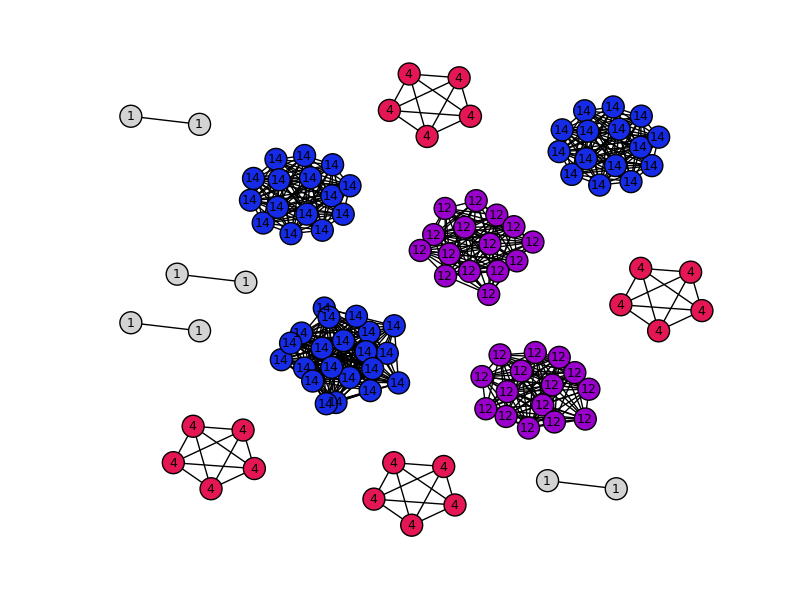
\includegraphics[scale=0.36]{figures/illustrative_aux_graph_3_candidates}
}
\hspace{.05in}
\subfloat[All subgraphs $H_{candidate}$ from $H_3$ computed using flow-based connectivity algorithm for local node connectivity.]{
\label{fig:aux3_cand_ex}
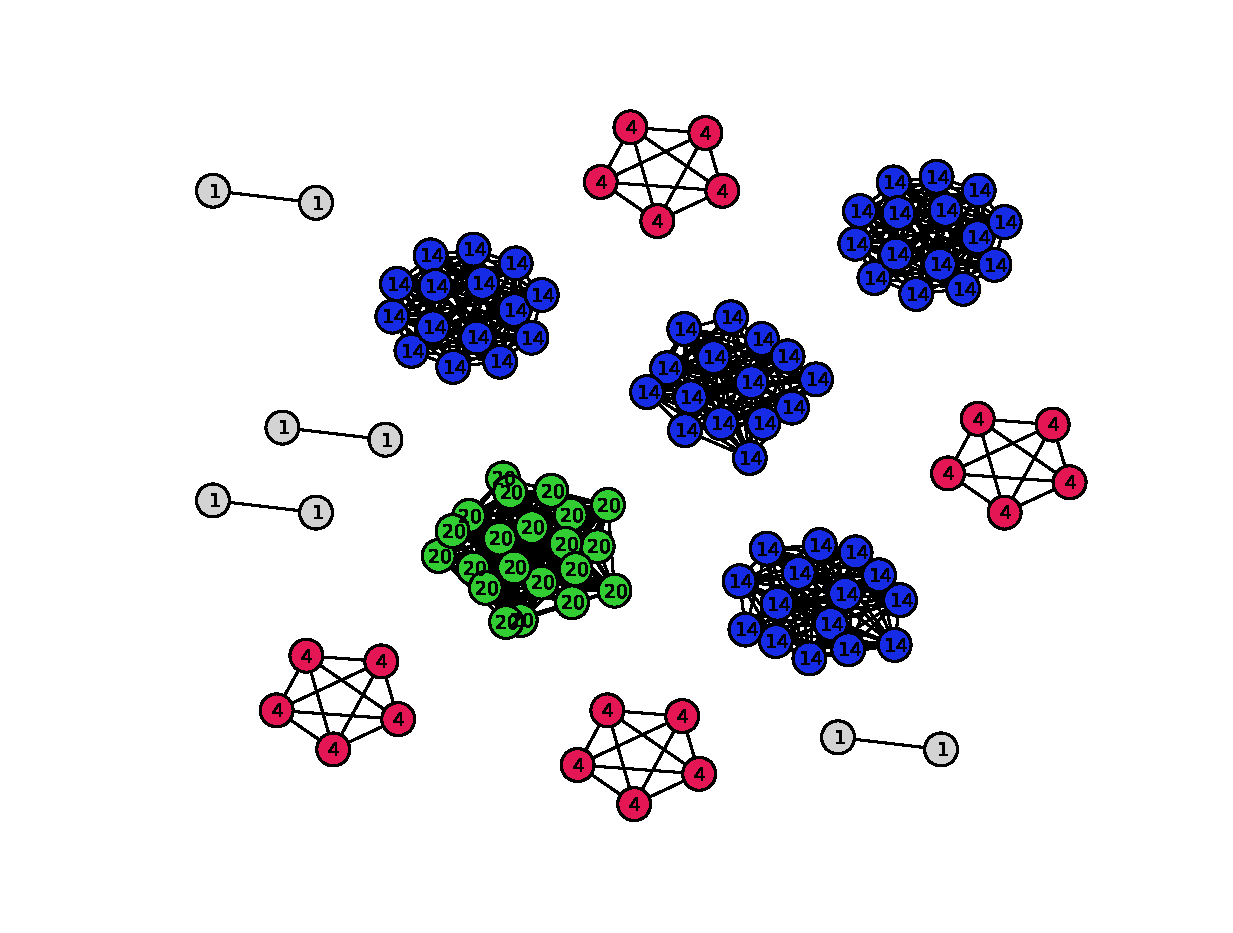
\includegraphics[scale=0.36]{figures/illustrative_aux_graph_3_candidates_exact}
}
\hspace{.05in}
\subfloat[Detected tri-components using the heuristics with the relaxation criteria of density $\ge 0.95$ in $H_{candidate}$.]{
\label{fig:subgraphs3}
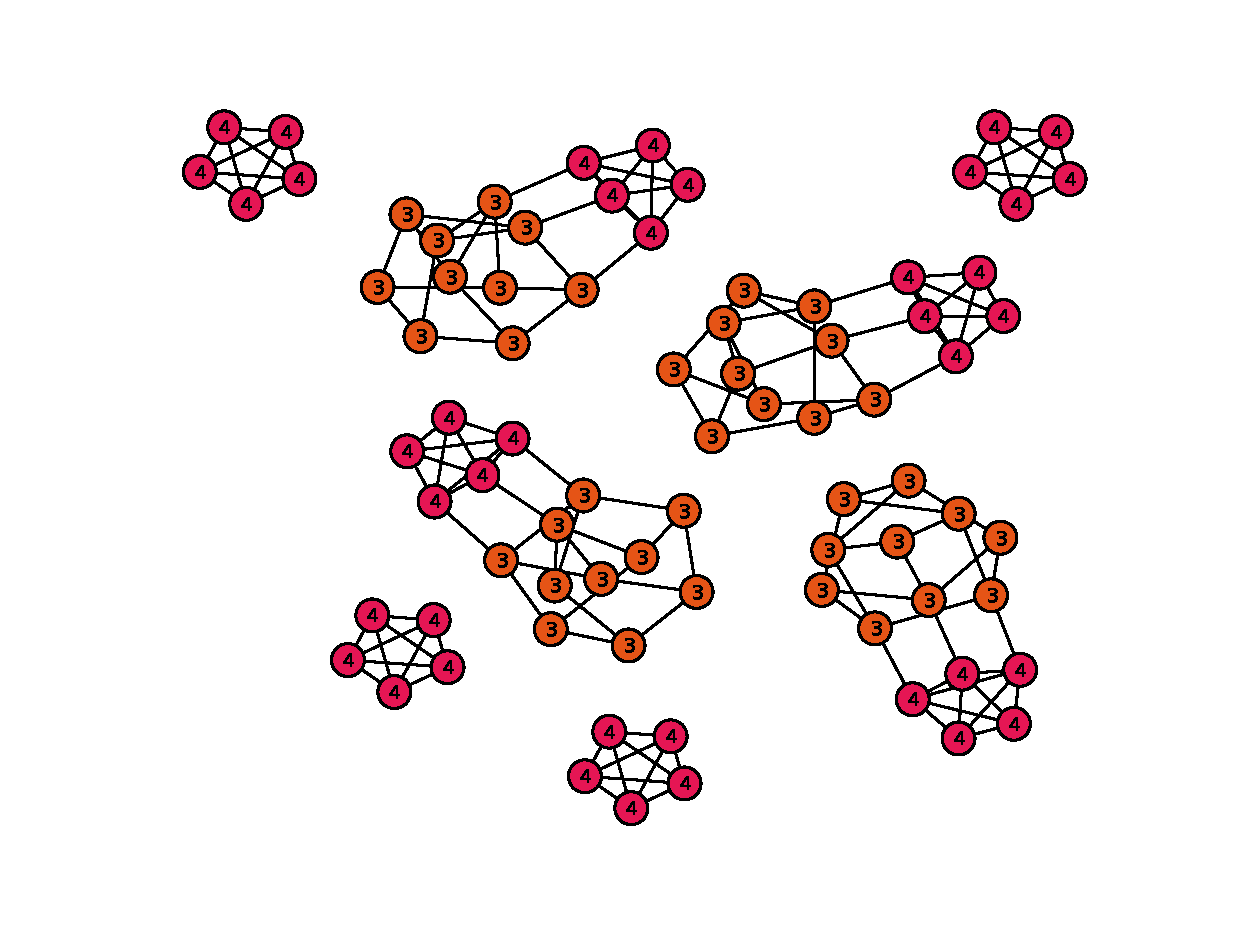
\includegraphics[scale=0.36]{figures/illustrative_candidates_3}
}
\hspace{.05in}

\caption[Auxiliary graph $H_3$ for $k=3$.]{Auxiliary graph $H_3$ for $k=3$. Note that when using White and Newman's approximation algorithm for local node connectivity (subfigure a), some node independent paths are not detected: the $P$ subgraphs linked to the two $K_5$ that overlap in two nodes should have core number 14 (blue) as in subfigure b, but they have core number 12. Thus to correctly detect all tricomponents we have to set a relaxation criteria for $H_{candidate}$, in this example setting density at 0.95 or allowing a variation of 2 in the degree of all nodes of $H_{candidate}$, allows the algorithm to correctly detect all tricomponents.}
\label{fig:example_3}
\end{figure}

%\end{landscape}


\begin{figure}[H]
\centering
\subfloat[Auxiliary graph $H$ for $k=4$ computed using White and Newman's approximation.]{
\label{fig:aux4}
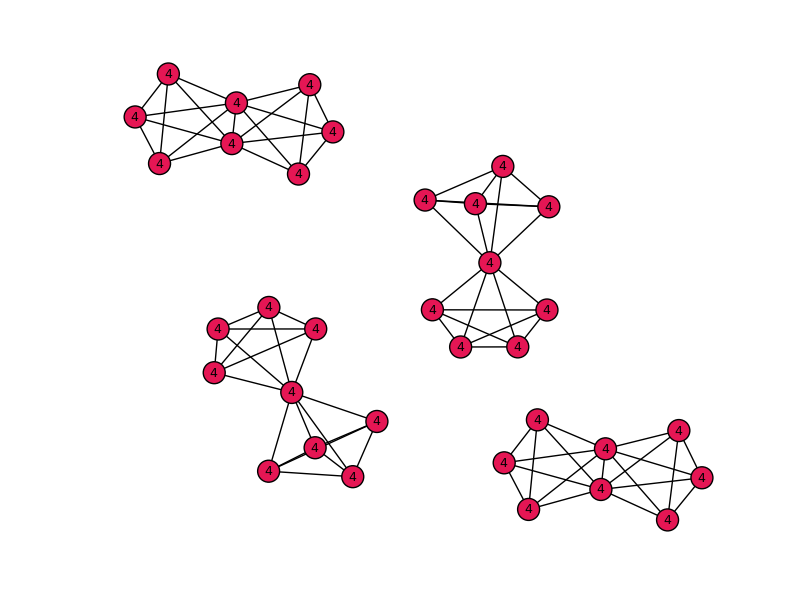
\includegraphics[scale=0.36]{figures/illustrative_aux_graph_4}
}
\hspace{.05in}
\subfloat[Detected 4-components using our heuristics. Note that there should be four more $K_5$, the ones that overlap in two nodes are not detected as 4-components. See text for an explanation.]{
\label{fig:subgraphs4}
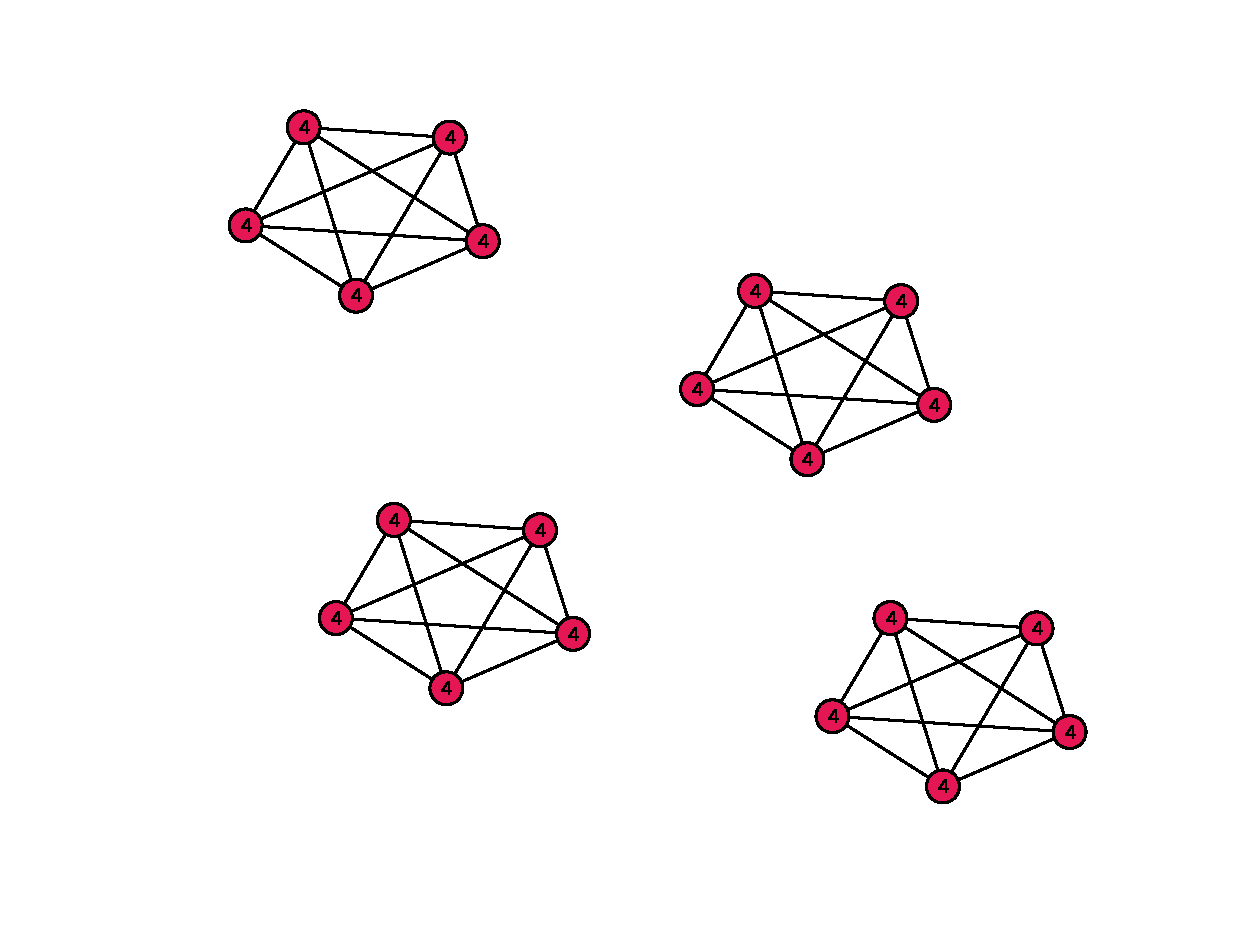
\includegraphics[scale=0.36]{figures/illustrative_candidates_4}
}

\caption[Auxiliary graph $H_4$ for $k=4$.]{Auxiliary graph $H_4$ for $k=4$. In this case both White and Newman's approximation algorithm, and the exact flow-based algorithm for local node connectivity yield equal results. Note that there should be four more $K_5$ in subfigure b, the ones that overlap in two nodes are not detected as 4-components. This is because, as can be seen in subfigure a, the nodes in these $H_{candidate}$ subgraphs have all the same core number, but their density is 0.67 and the difference in degree is 3. Thus, in order to detect them we would have to relax the clique criteria for $H_{candidate}$ too much, and even then we would classify both $K_5$ as a single 4-component, which is obviously wrong.}
\label{fig:example_4}
\end{figure}

As discussed above, a $k$-core is a maximal subgraph that contains nodes of degree $k$ or more. The core number of a node is the largest value $k$ of a $k$-core containing that node. On the other hand, a $k$-component is a maximal subgraph that cannot be disconnected by removing less than $k$ nodes. The component number of a node is the largest value $k$ of a $k$-component containing that node.

The graph of figure \ref{fig:example} is a biconnected 3-core, which means that it is a graph with minimum degree $=3$ that cannot be disconnected by removing less than 2 nodes. Our algorithm starts by considering the whole graph the step 2, but in $k$-core subgraphs with more than one bicomponent, the following steps are performed for each bicomponent of the $k$-core. We will only compute up until $k=4$ because the largest core number of a node in $G$ is 4. 

For $k=3$ we create an auxiliary graph with all biconnected nodes with core number $\ge 3$ (see figure \ref{fig:example_3}). In this case all nodes have a core number greater than or equal to 3. Thus the auxiliary graph $H$ for $k=3$ contains all 99 nodes. We then link two nodes in $H_3$ if we can find $k$ or more node independent paths between them. As we can see, the result are five connected components, four of which correspond to each Petersen graph plus the two $K_5$, while the last one corresponds to the nodes that form the grid. The later has 4 nodes that are linked by 3 node independent paths to only one node, these four nodes are the four corner nodes of the grid. 

Notice that when using White and Newman's approximation algorithm for local node connectivity (subfigure \ref{fig:aux3}), some node independent paths that actually exist are not detected: the $P$ subgraphs linked to the two $K_5$ that overlap in two nodes should have a core number of 14 (blue) because there are 3 node independent paths linking each pair of different nodes in the subgraph formed by the $P$ and the $K_5$ to which it is linked through three edges, as in subfigure \ref{fig:aux3_ex}, which was computed using the exact flow-based algorithm for local node connectivity. Notice also that the grid has core number 14 in \ref{fig:aux3} but actually should be core number 20 as shown in \ref{fig:aux3_ex}. This illustrates the importance of computing biconnected components of $H$ (step 3.c) before building the subgraphs $H_{candidate}$ (step 3.d).

Figures \ref{fig:aux3_cand} and \ref{fig:aux3_cand_ex} depict $H_{candidate}$ subgraphs, the former using White and Newman's approximation algorithm and the latter using an exact flow-based algorithm for local node connectivity. The subgraphs $H_{candidate}$ are composed by nodes that are in the same biconnected component of $H$ and have \emph{exactly} the same core number. Notice that in figure \ref{fig:aux3_cand} the $P$ graphs linked to the two $K_5$ that overlap in two nodes have core number $< n-1$ (the magenta clusters), thus they are not complete (density=0.96) and the degree of their nodes is not homogeneous: two nodes have degree 12, four have degree 13, and nine have degree 14. Therefore, if we enforce the clique criteria for $H_{candidate}$ we would not detect all tricomponents because, following the algorithm, we would have to start removing nodes with the lowest degree and check if at some point we find a complete subgraph. In order to correctly detect all tricomponents in this illustrative example, we have to first establish a relaxation for the clique criteria for $H_{candidate}$. In this case, setting density at 0.95 or allowing a variation of 2 in the degree of all nodes of $H_{candidate}$, allows the algorithm to correctly detect all tricomponents as shown in figure \ref{fig:subgraphs3}.

For $k=4$, the auxiliary graph $H_4$ is composed of 4 connected components which correspond to the pairs of $K_5$ that share one node and the pairs of $K_5$ that share 2 nodes (see figure \ref{fig:aux4}). In terms of biconnectivity, there are six bicomponents, with the two $K_5$ that overlap in two nodes as a single bicomponent. Inside these six bicomponents there are eight 4-components, but only four of them were detected (see figure \ref{fig:subgraphs4}). This is because when we build the $H_{candidate}$ subgraphs with all nodes in each biconnected component of $H_4$ that have exactly the same core number, in the case of the two $K_5$ that overlap in two nodes, all their nodes  have the same core number (4), but their density is 0.67 and the difference in degree is 3. Thus, in order to detect them we would have to relax the clique criteria for $H_{candidate}$ too much, and even then, we would classify both $K_5$ overlapping in two nodes as a single 4-component, which is obviously wrong because they have node connectivity 2.

Note that this kind of false negative only happens when two $k$-components of the same level of connectivity and the same order overlap. If instead of two $K_5$ they were $k$-components with different order but the same connectivity, our algorithm would be able to separate them because they would have a different core number and thus they would be part of a different $H_{candidate}$ subgraph.

\newpage

\section{Performance analysis}
\label{performance}

The heuristics presented here are implemented on top of NetworkX \citep{hagberg:2008}, a library for the analysis of complex networks, using the Python programming language \citep{vanrossum:1995}. We have chosen Python because it is a language with high readability and flexibility that allows you to easily apply the well know principle of writing software for people to read and, only incidentally, for machines to execute \citep{abelson:1985}. To ensure reproducibility and accessibility we have used only free software to build and run all analyses presented in this paper. 

The implementation of the heuristics presented here is not trivial; a careful implementation is needed to ensure that it has a reasonable memory footprint and that it runs in a reasonable time. Appendix C contains a detailed discussion of the implementation details and appendix D contains the python code of a simplified implementation for illustrative purposes.

\begin{figure}[h]
\centering
\subfloat[Performance of connectivity algorithms when adding nodes maintaining constant the average degree (Erdös-Rènyi) or the exponent of the power law governing the degree distribution ($\alpha=2$). Logarithmic scale.]{
\label{fig:nodes}
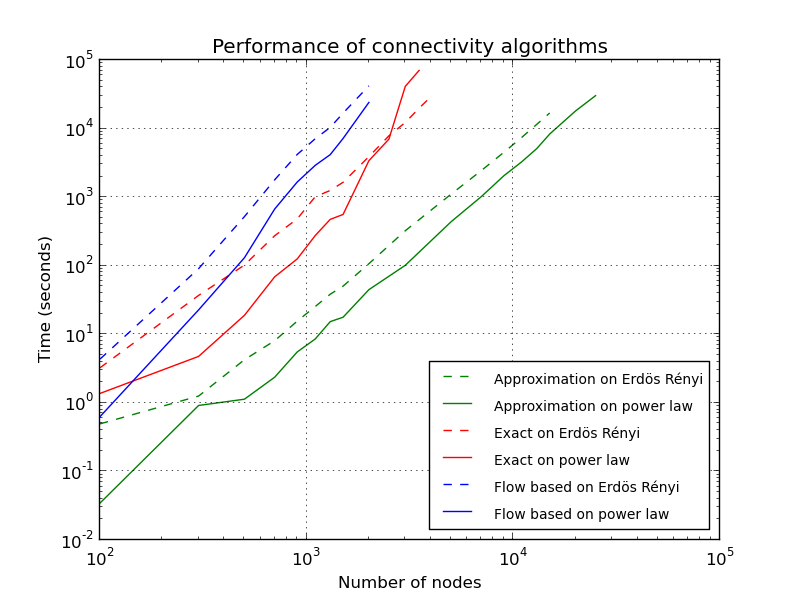
\includegraphics[scale=0.37]{figures/node_performance_log}
}
\hspace{.05in}
\subfloat[Performance of the heuristics when adding edges and maintaining nodes constant (1000 nodes). Inset: performance of the exact algorithm with one order of magnitude fewer nodes (100 nodes). Both in logarithmic scale.]{
\label{fig:edges}
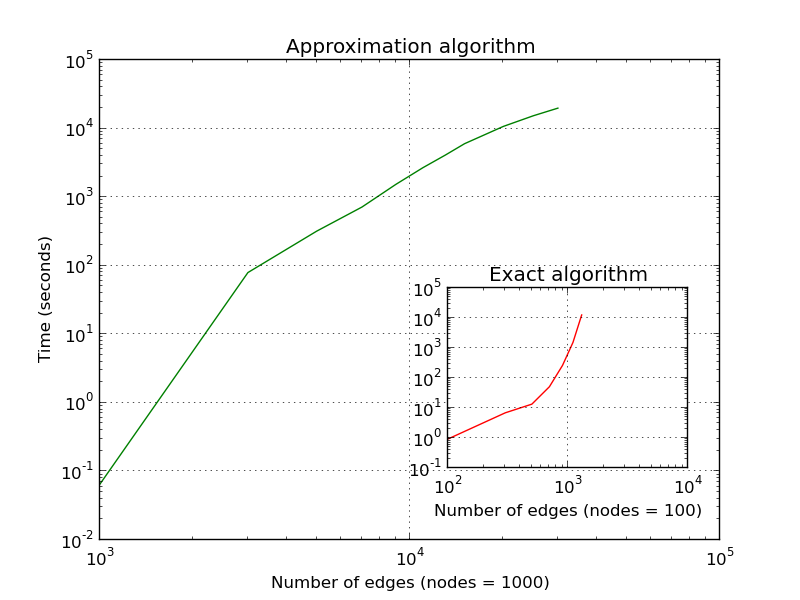
\includegraphics[scale=0.37]{figures/edge_performance_log}
}
%\hspace{.2in}

\begin{minipage}{\textwidth}
\caption[Loglog plots for comparing between heuristics and exact algorithms]{Log-log plots for comparing between the heuristics and the exact algorithm to compute $k$-component structure. In this comparison, the heuristics do not compute the average node connectivity, only plain node connectivity, which is what is calculated by the exact algorithm. We have also implemented the exact algorithm in order to be able to compare both algorithms using the same language and infrastructure. All figures presented here were obtained running PyPy \citep{bolz:2009}. Using the heuristics proposed in this paper, we are able to handle networks almost one order of magnitude bigger than with the exact algorithm.}
\label{fig:performance}
\end{minipage}
\end{figure}

Figure \ref{fig:performance} presents the performance of the heuristics (green) compared with two variants of the exact algorithm: the Moody \& White algorithm based on $k$-cutsets (red) and our algorithm using exact flow-based node connectivity for building the auxiliary graph. The tests were performed, on the one hand, on random graphs with fixed average degree (Erdös-Renyi model) and fixed power law exponent (Power law model) of several different orders. And, on the other hand, for graphs with a fixed number of nodes (1000 for the heuristics and 100 for the exact) where we increase the number of edges. Random networks built using the Erdös-Renyi model have a flat hierarchical structure because edges are evenly distributed across all nodes of the network. The Erdös-Renyi graphs used in this benchmark have a big tricomponent and no higher connectivity levels. Random networks built using a power law based degree distribution have a steep hierarchical structure, the networks used in the benchmark have hierarchy levels of up to 20. Both the heuristics and the exact algorithms perform better in sparse networks with a steep hierarchical structure.

As we can see in figure \ref{fig:performance} the heuristics runs in polynomial time. It is fast enough to be practically applicable to networks with a few tens of thousands of nodes and edges. This is one order of magnitude better than the exact algorithm proposed by \citet{moody:2003}, and also an order of magnitude faster than using flow-based algorithms for building the auxiliary graph. Notice that the $k$-cutset based algorithm proposed by Moody \& White (or at least our implementation) is faster than the exact flow-based local node connectivity variant of our algorithm.

The implementation that we provide in this paper only considers the exact solution for biconnected components. The heuristics presented here uses biconnectivity, but can be improved by using a triconnectivity algorithm. It would be: a) faster because there is a linear algorithm to compute triconnected components \citep{tarjan:1974,gutwenger:2001}; and, b) more accurate, because we compute the exact solution up to $k=3$. But, as far as we know, there is no publicly available implementation of triconnected components. An optimal implementation of the heuristics presented here would have to incorporate the triconnectivity algorithm to improve its accuracy and to allow it to run in reasonable time on somewhat larger networks.

\newpage

\section{Implementation details}
\label{implementation}

The implementation of the heuristics proposed here was done by the first author listed on the NetworkX python library \citep{hagberg:2008}, a Python package for the study of the structure and dynamics of complex networks. Other parts of the powerful Python \citep{vanrossum:1995} scientific computing stack \citep{scipy,ipython, hunter:2007} were also essential. The main requirement was that the whole software stack must be free software in order to avoid the black box effect of software solutions that do not release their source code. We believe that this is a necessary condition for ensuring the reproducibility of scientific research. Appendix B contains python code for the main part of the algorithm. 

The implementation of the heuristics is not trivial. There are a few questions that need to be addressed in order to obtain a performance ---both in terms of computation time and memory consumption--- that will allow for these heuristics to be applied to large networks. The authors are in-debted to Aric Hagberg and Dan Schult (developers of the NetworkX package) for their help in this implementation.

The second step of the heuristics (compute the biconnected components of the input graph and use them as a baseline for $k$-components with $k > 2$) is faster than using the logic of the heuristics for $k=2$. Biconnected components computation runs in linear time in respect to the number of nodes and edges \citep{tarjan:1972}. Besides in large networks, bicomponents are formed by an important part of the nodes of the network. Thus if we use the approximation logic to compute them, the memory footprint for large networks is too large to be practical. The implementation provided with this paper only computes the exact solution for bicomponents but there is also a linear algorithm to compute triconnected components \citep{tarjan:1974,gutwenger:2001}. The heuristics would be even faster if we applied the approach used for bicomponents to that of tricomponents. But the implementation of triconnectivity is quite challenging and, to our knowledge, there is no implementation of triconnected components in free network analysis software packages.

The auxiliary graph $H$ is usually very dense in real world networks because a large part of nodes that are in a biconnected part of a $k$-core are actually part of a $k$-component. The memory footprint of creating this dense auxiliary graph prevents a naive implementation of the heuristics in order to be practical for large networks. Our solution for this problem is to use a complement graph data structure that only stores information on the edges that are \emph{not} present in the actual auxiliary graph. When applying algorithms to this complement graph data structure, it behaves as if it were the dense version. This is the only way to have a memory footprint that will allow for the application of the heuristics presented in this paper to large networks.

\newpage

\section{Python code}
\label{code}

We provide a git repository with all the data, code, results, and other materials related to this paper at \href{https://github.com/jtorrents/structural_cohesion}{https://github.com/jtorrents/structural\_cohesion}.

We also contributed our implementation of the exact algorithm for finding $k$-components, and the heuristics that we propose here, to NetworkX a free software Python package for the analysis of complex networks. The relevant code and documentation can be found at:

\begin{itemize}

\item Kanevsky’s algorithm for finding all minimum-size node cut-sets:

\begin{scriptsize}

\begin{description}

\item[docs:] \href{http://networkx.readthedocs.org/en/latest/reference/generated/networkx.algorithms.connectivity.kcutsets.all_node_cuts.html}{http://networkx.readthedocs.org/en/latest/reference/generated/networkx.algorithms.connectivity.kcutsets.all\_node\_cuts.html}

\item[code:] \href{https://github.com/networkx/networkx/blob/master/networkx/algorithms/connectivity/kcutsets.py}{https://github.com/networkx/networkx/blob/master/networkx/algorithms/connectivity/kcutsets.py}

\end{description}

\end{scriptsize}

\item Moody and White exact algorithm:

\begin{scriptsize}

\begin{description}

\item[docs:] \href{http://networkx.readthedocs.org/en/latest/reference/generated/networkx.algorithms.connectivity.kcomponents.k_components.html}{http://networkx.readthedocs.org/en/latest/reference/generated/networkx.algorithms.connectivity.kcomponents.k\_components.html}

\item[code:] \href{https://github.com/networkx/networkx/blob/master/networkx/algorithms/connectivity/kcomponents.py}{https://github.com/networkx/networkx/blob/master/networkx/algorithms/connectivity/kcomponents.py}

\end{description}
\end{scriptsize}

\item White and Newman approximation for node connectivity:

\begin{scriptsize}
\begin{description}

\item[docs:] \href{http://networkx.readthedocs.org/en/latest/reference/generated/networkx.algorithms.approximation.connectivity.node_connectivity.html}{http://networkx.readthedocs.org/en/latest/reference/generated/networkx.algorithms.approximation.connectivity.node\_connectivity.html}

\item[code:] \href{https://github.com/networkx/networkx/blob/master/networkx/algorithms/approximation/connectivity.py}{https://github.com/networkx/networkx/blob/master/networkx/algorithms/approximation/connectivity.py}

\end{description}
\end{scriptsize}

\item Our heuristics for computing $k$-components:

\begin{scriptsize}
\begin{description}

\item[docs:] \href{ttp://networkx.readthedocs.org/en/latest/reference/generated/networkx.algorithms.approximation.kcomponents.k_components.html}{ttp://networkx.readthedocs.org/en/latest/reference/generated/networkx.algorithms.approximation.kcomponents.k\_components.html}

\item[code:] \href{https://github.com/networkx/networkx/blob/master/networkx/algorithms/approximation/kcomponents.py}{https://github.com/networkx/networkx/blob/master/networkx/algorithms/approximation/kcomponents.py }

\end{description}
\end{scriptsize}

\end{itemize}

We also add here a simplified implementation of the heuristics for illustrative purposes.

\newpage

\begin{scriptsize}
\begin{lstlisting}
# Standard python libraries
import itertools
import collections
# NetworkX library for network analysis
import networkx as nx
# AntiGraph data structure
# see https://github.com/networkx/networkx/blob/master/examples/subclass/antigraph.py

def k_components(G, average=True, exact=False, min_density=0.95):
    # Dictionary with connectivity level (k) as keys and a list of
    # sets of nodes that form a k-component as values
    k_components = collections.defaultdict(list)
    # make a few functions local for speed
    node_connectivity = local_node_connectivity
    k_core = nx.k_core
    core_number = nx.core_number
    biconnected_components = nx.biconnected_components
    density = nx.density
    combinations = itertools.combinations
    # Exact solution for k = {1,2}
    # There is a linear time algorithm for triconnectivity, if we had an
    # implementation available we could start from k = 4.
    for component in  nx.connected_components(G):
        # isolated nodes have connectivity 0
        comp = set(component)
        if len(comp) > 1:
            k_components[1].append(comp)
    for bicomponent in  nx.biconnected_components(G):
        # avoid considering dyads as bicomponents
        bicomp = set(bicomponent)
        if len(bicomp) > 2:
            k_components[2].append(bicomp)
    # There is no k-component of k > maximum core number
    # \kappa(G) <= \lambda(G) <= \delta(G)
    g_cnumber = core_number(G)
    max_core = max(g_cnumber.values())
    for k in range(3, max_core + 1):
        C = k_core(G, k, core_number=g_cnumber)
        for nodes in biconnected_components(C):
            # Build a subgraph SG induced by the nodes that are part of
            # each biconnected component of the k-core subgraph C.
            if len(nodes) < k:
                continue
            SG = G.subgraph(nodes)
            # Build auxiliary graph
            H = _AntiGraph()
            H.add_nodes_from(SG.nodes())
            for u,v in combinations(SG, 2):
                K = node_connectivity(SG, u, v, cutoff=k)
                if k > K:
                    H.add_edge(u,v)
            for h_nodes in biconnected_components(H):
                if len(h_nodes) <= k:
                    continue
                SH = H.subgraph(h_nodes)
                for Gc in _cliques_heuristic(SG, SH, k, min_density):
                    for k_nodes in biconnected_components(Gc):
                        Gk = nx.k_core(SG.subgraph(k_nodes), k)
                        if len(Gk) <= k:
                            continue
                        k_components[k].append(set(Gk))
    return k_components


def _cliques_heuristic(G, H, k, min_density):
    h_cnumber = nx.core_number(H)
    for i, c_value in enumerate(sorted(set(h_cnumber.values()), reverse=True)):
        cands = set(n for n, c in h_cnumber.items() if c == c_value)
        # Skip checking for overlap for the highest core value
        if i == 0:
            overlap = False
        else:
            overlap = set.intersection(*[
                        set(x for x in H[n] if x not in cands)
                        for n in cands])
        if overlap and len(overlap) < k:
            SH = H.subgraph(cands | overlap)
        else:
            SH = H.subgraph(cands)
        sh_cnumber = nx.core_number(SH)
        SG = nx.k_core(G.subgraph(SH), k)
        while not (_same(sh_cnumber) and nx.density(SH) >= min_density):
            SH = H.subgraph(SG)
            if len(SH) <= k:
                break
            sh_cnumber = nx.core_number(SH)
            sh_deg = dict(SH.degree())
            min_deg = min(sh_deg.values())
            SH.remove_nodes_from(n for n, d in sh_deg.items() if d == min_deg)
            SG = nx.k_core(G.subgraph(SH), k)
        else:
            yield SG
\end{lstlisting}
\end{scriptsize}

\newpage

\section{Accuracy and limitations of the heuristics}
\label{accuracy}

Figure \ref{fig:accuracy} shows the accuracy of connectivity structure detected by the heuristics for all empirical networks. In the subfigures, green bars are $k$-components with node connectivity $\ge k$ and red bars represent $k$-components with node connectivity $< k$.  Note that, once we have an approximate structure of $k$-components, we can check ---in a reasonable time frame--- if the resulting $k$-components actually have node connectivity $k$ using flow based connectivity algorithms \citep[chapter 7]{brandes:2005}. For the candidate $k$-components that turned out to have node connectivity lower than $k$, we used the exact algorithm proposed by \citet{moody:2003} to find out the order and size of the actual $k$-components inside the candidate $k$-component detected using our heuristics.

\begin{figure}[p]
\centering
\subfloat[Bipartite network formed by developers and packages over 2 years of collaboration (from 2007 to 2009) on the release codenamed Lenny of the Debian operating system]{
\label{fig:lenny2m}
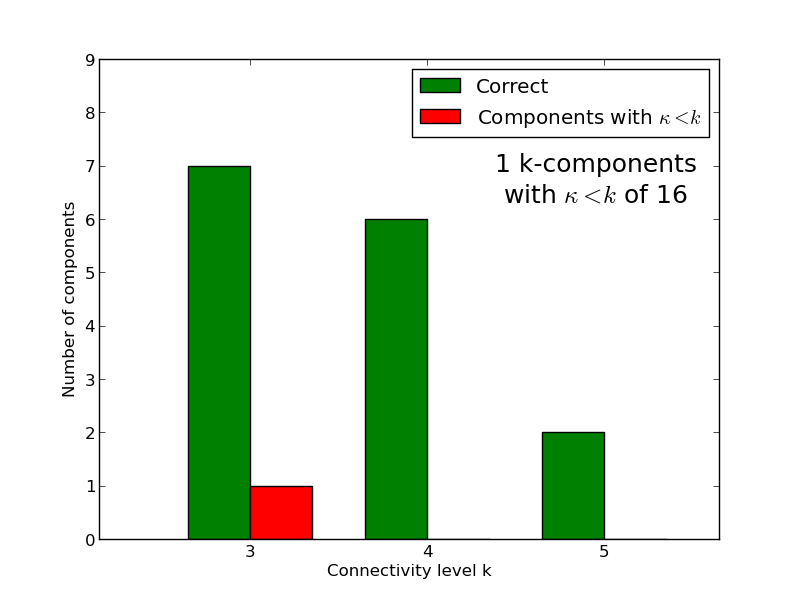
\includegraphics[scale=0.35]{figures/accuracy_lenny_2mode}
}
\hspace{.05in}
\subfloat[Unipartite network formed by developers over 2 years of collaboration (from 2007 to 2009) on the release codenamed Lenny of the Debian operating system]{
\label{fig:lenny1m}
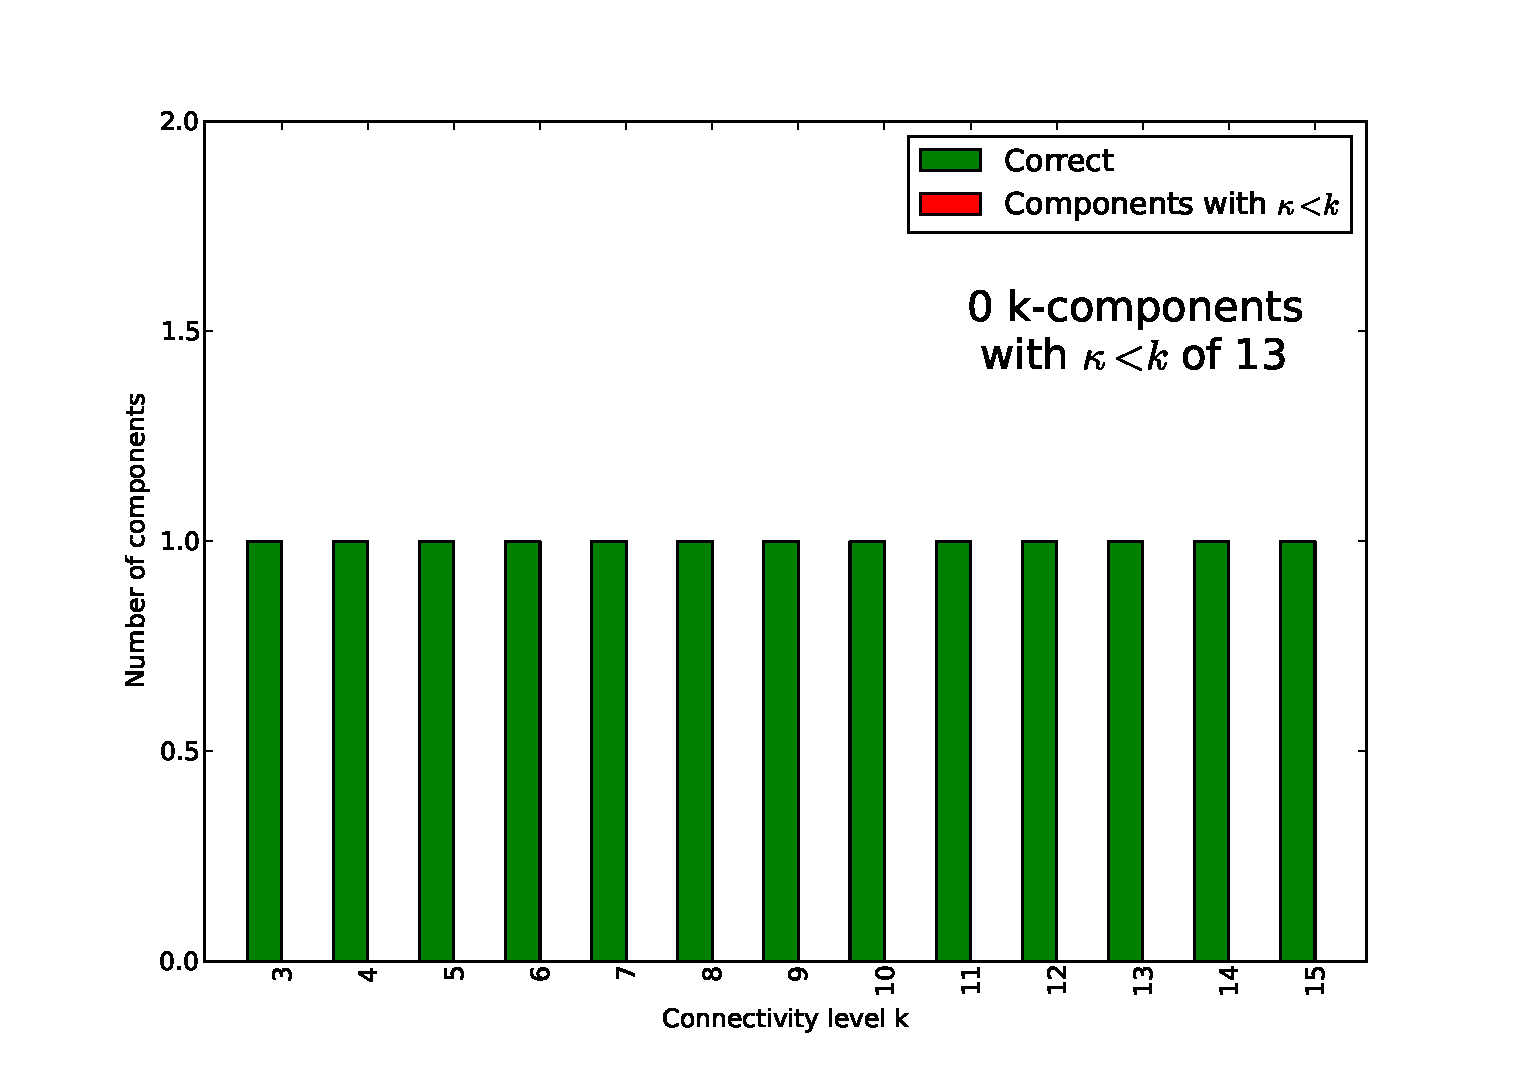
\includegraphics[scale=0.27]{figures/accuracy_lenny_1mode}
}
\hspace{.01in}
\subfloat[Bipartite network formed by scientists and preprints during a five-year period (2006-2010) in the high energy physics (theory) section of arXiv.org]{
\label{fig:hep_th_2m}
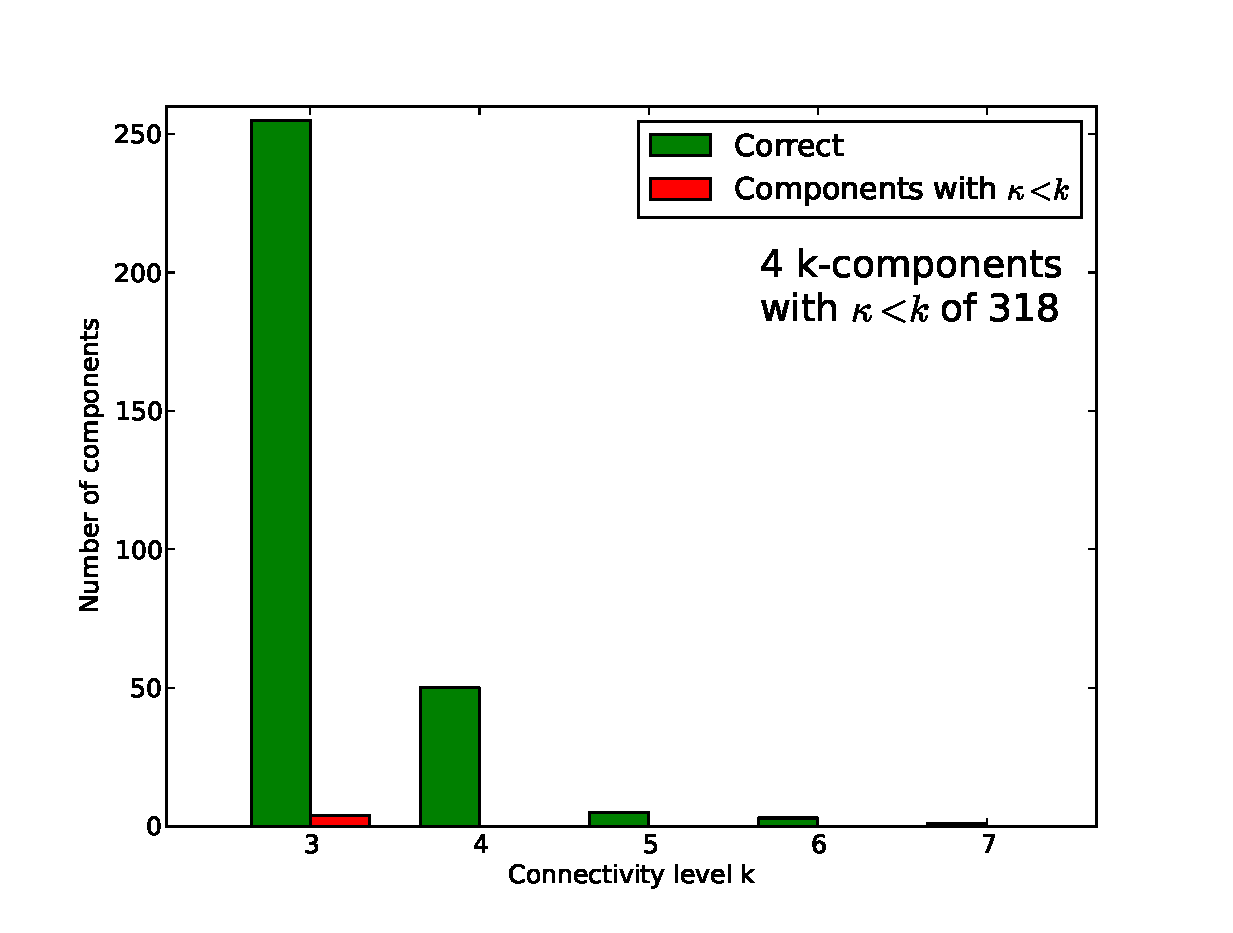
\includegraphics[scale=0.35]{figures/accuracy_hep_th_2mode}
}
\hspace{.05in}
\subfloat[Unipartite network formed by scientists during a five-year period (2006-2010) in the high energy physics (theory) section of arXiv.org]{
\label{fig:hep_th_1m}
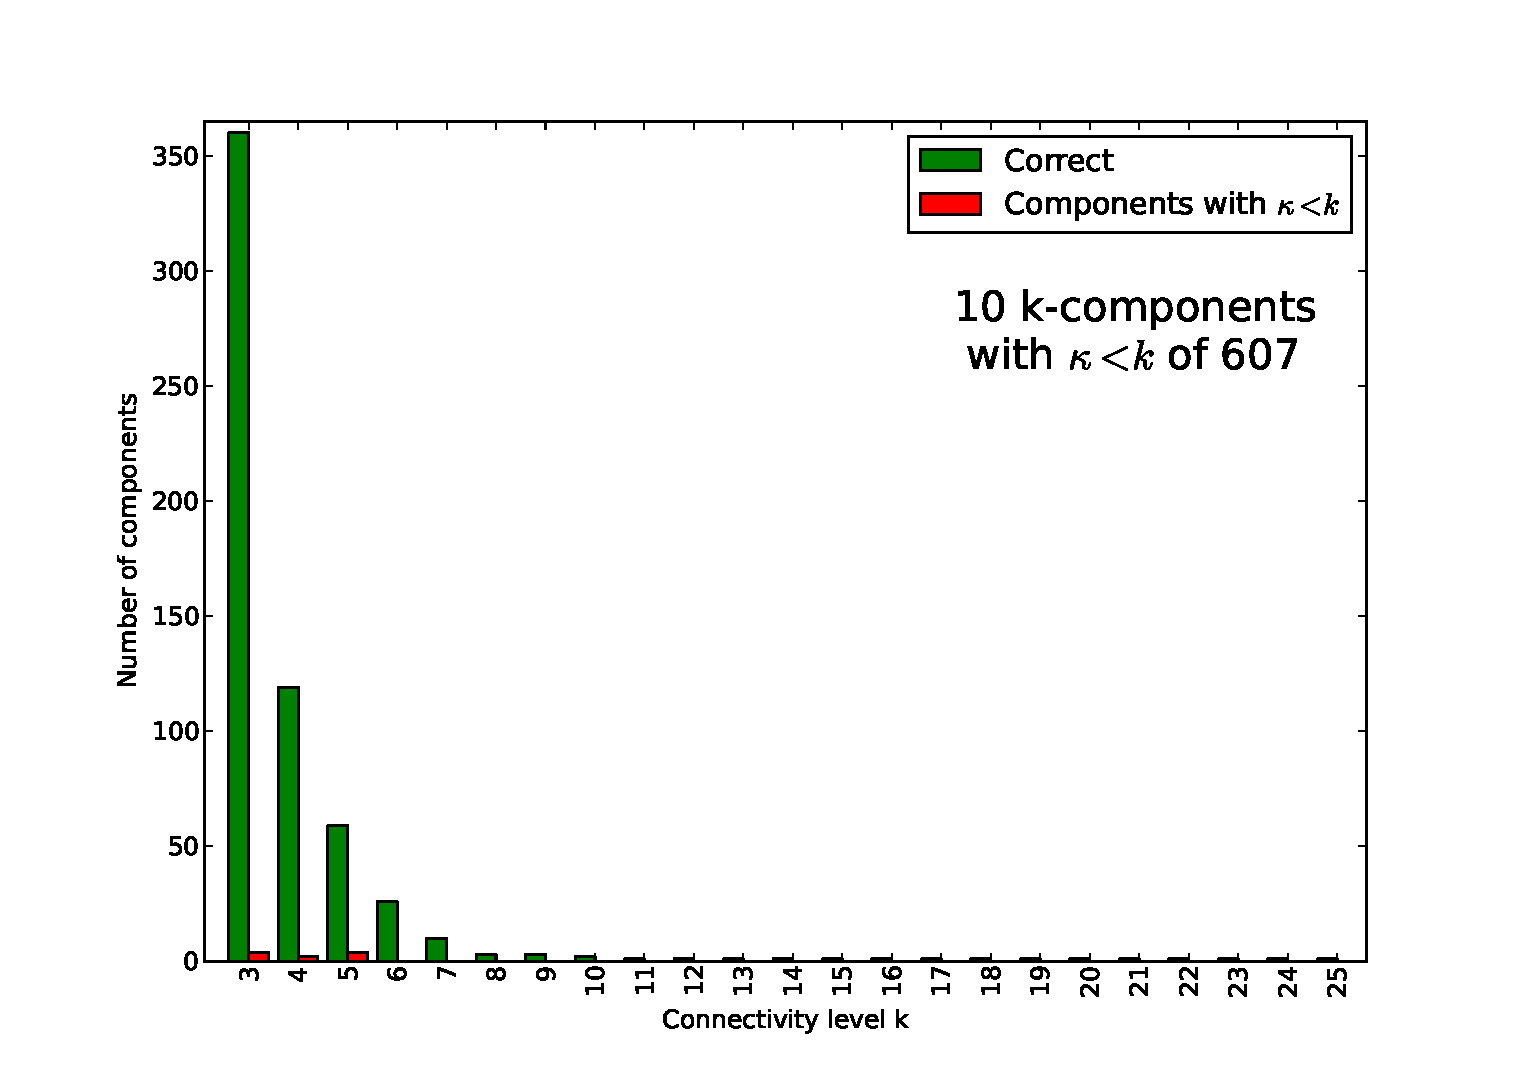
\includegraphics[scale=0.30]{figures/accuracy_hep_th_1mode}
}
\hspace{.01in}
\subfloat[Bipartite network formed by scientists and preprints during a five-year period (2006-2010) in the nuclear physics (theory) section of arXiv.org]{
\label{fig:nucl_th_2m}
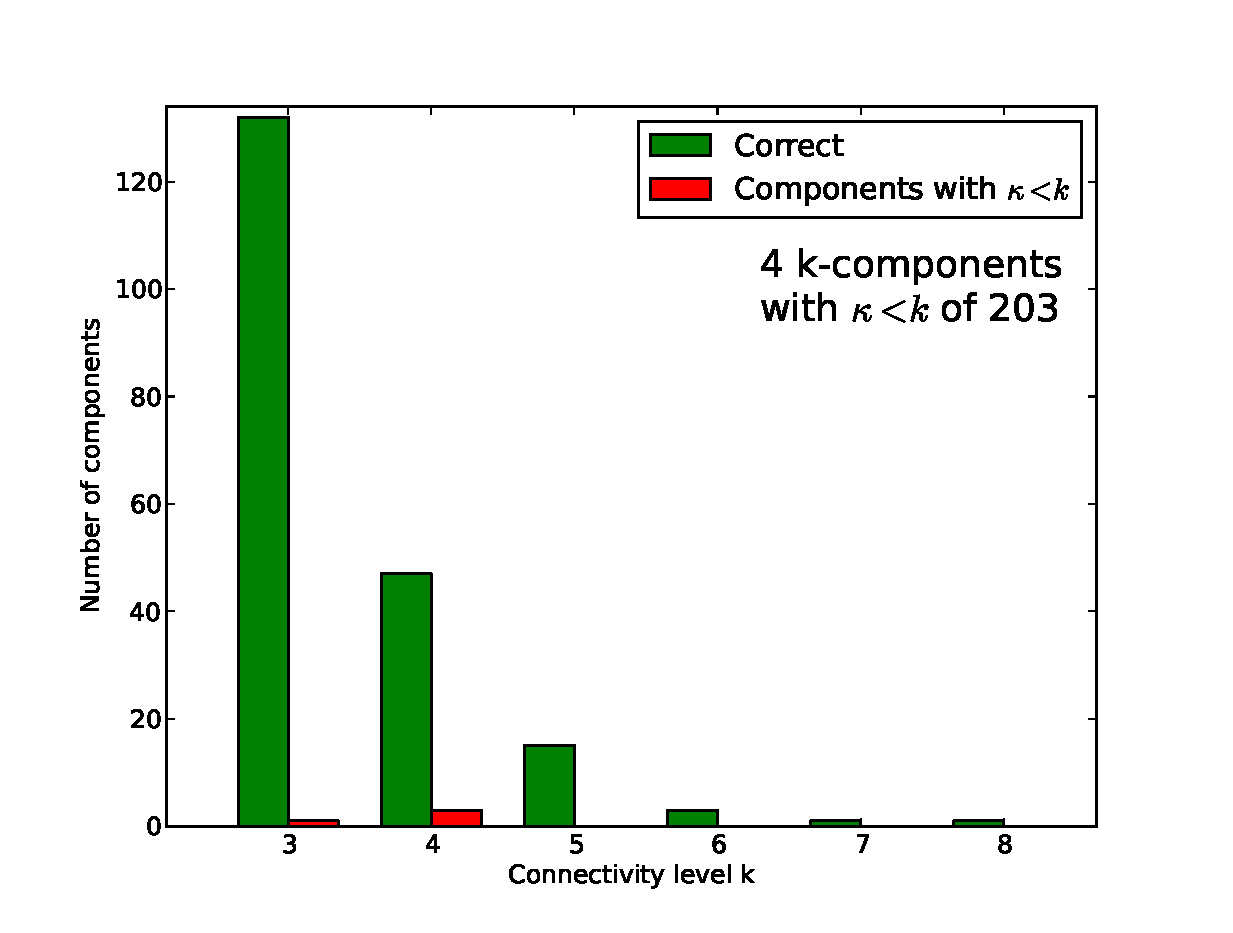
\includegraphics[scale=0.34]{figures/accuracy_nucl_th_2mode}
}
\hspace{.05in}
\subfloat[Unipartite network formed by scientists during a five-year period (2006-2010) in the nuclear theory section of arXiv.org]{
\label{fig:nucl_th_1m}
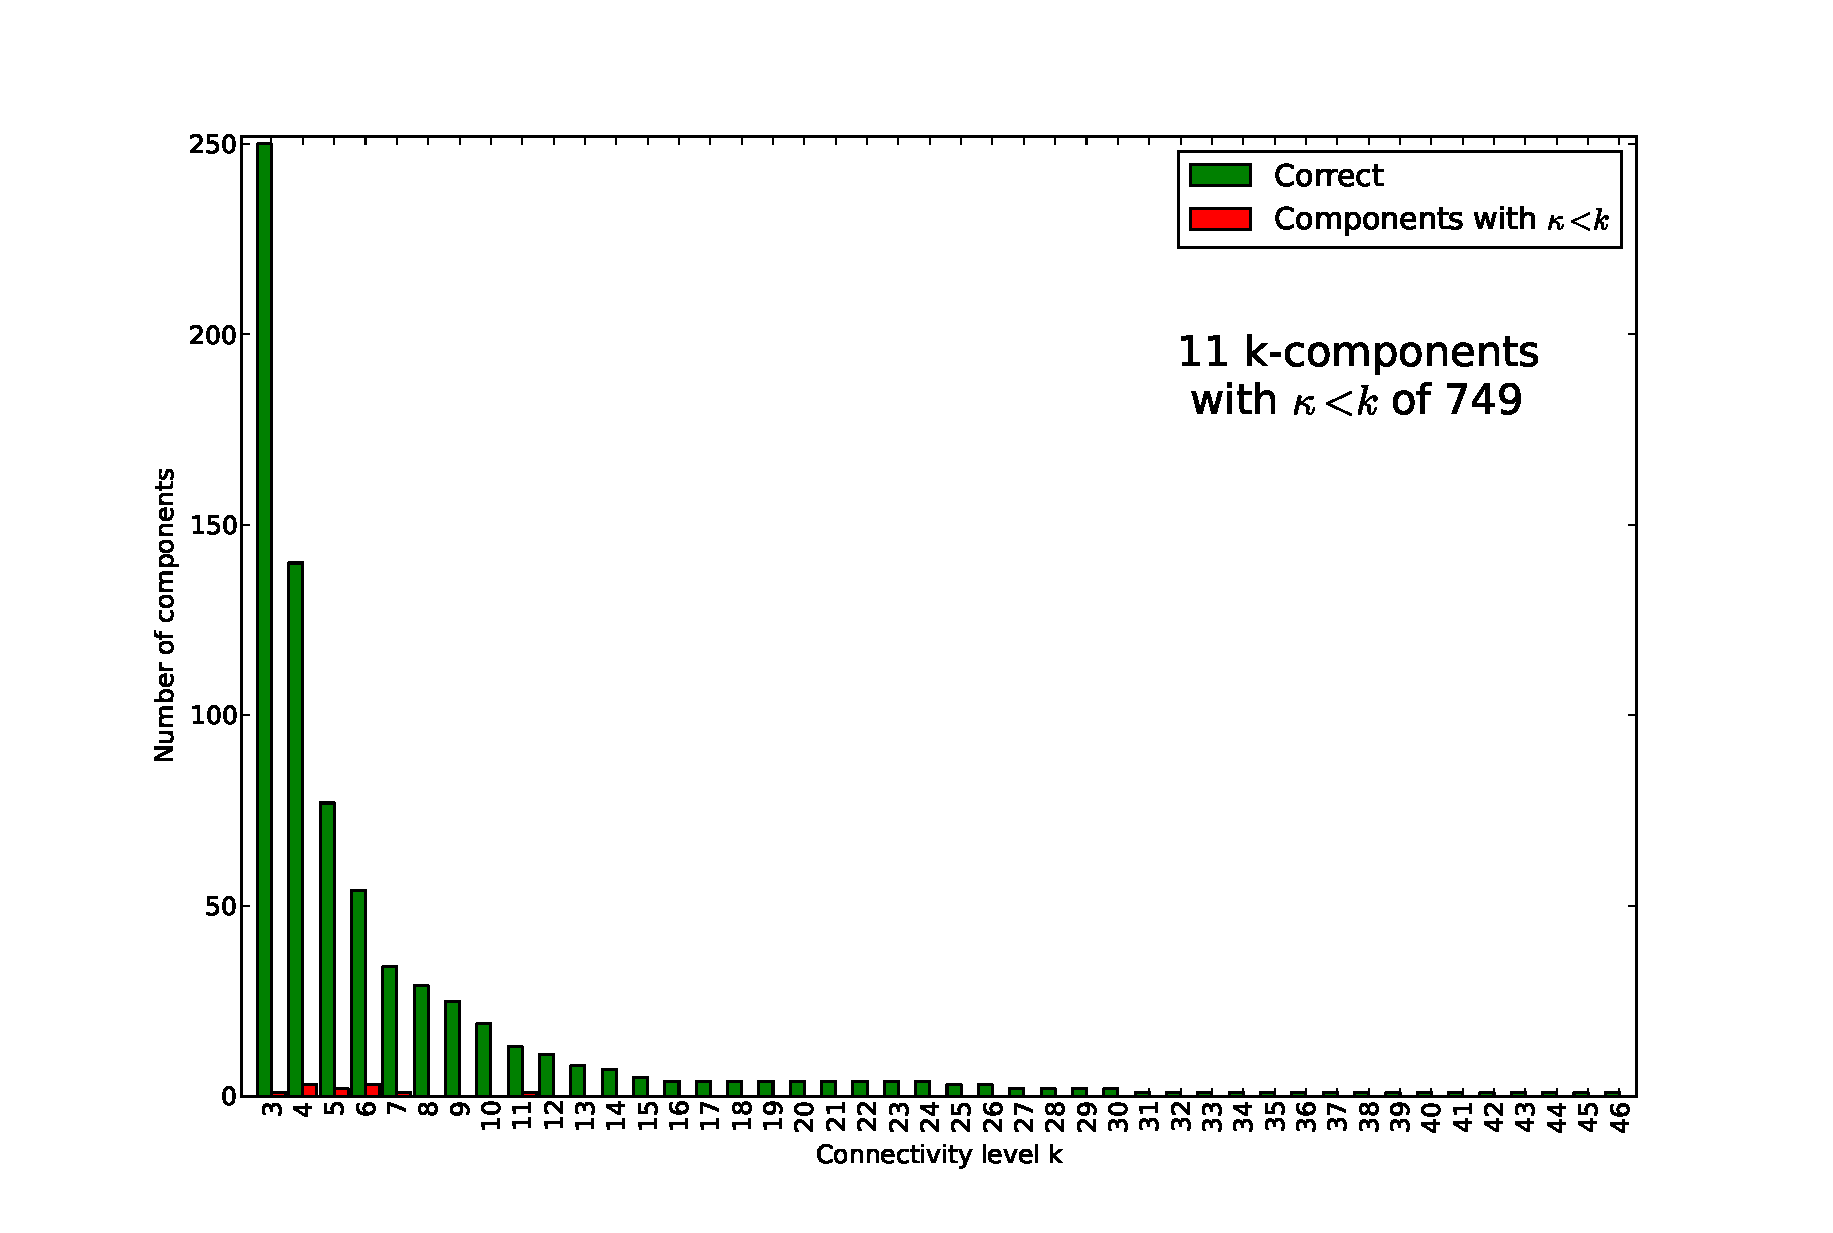
\includegraphics[scale=0.26]{figures/accuracy_nucl_th_1mode}
}
\caption[Accuracy barplots for the heuristics.]{Accuracy barplots. Green bars are $k$-components with node connectivity $\ge k$ and red bars represent $k$-components with node connectivity $< k$.}
\label{fig:accuracy}
\end{figure}

The output of our heuristics is an approximation to $k$-components based on computing extra-cohesive blocks for each biconnected component of all core levels of the network. Recall that in $k$-components all $k$ node independent paths go through nodes that belong to the $k$-component, but in extra-cohesive blocks some of the node independent paths may go through external nodes. Thus, there is no guarantee that the extra-cohesive blocks, even those that also form a $k$-core subgraph in $G$, have node connectivity $\kappa = k$. This is a source of false positives for the approximation of the $k$-component structure of a network. However, the results shown in figure \ref{fig:accuracy} suggest that the heuristics yield a good approximation for the actual ---$k$-component based--- cohesion structure of empirical networks.

If we consider all components of all sizes, as in figure \ref{fig:accuracy}, only a few of the extra-cohesive blocks detected by the heuristics have node connectivity of less than $k$, ranging from 6.5\% (a single component) in the case of Debian to 1.2\% of the components in the case of two-mode Nuclear Theory network. However, the extra-cohesive blocks that do not have the sufficient connectivity to be considered a $k$-component are, in the empirical networks analyzed, big components of levels \{3,4\}. This is because, in such big- and low-level components, a few node independent paths going through nodes that are part of the biconnected component of a $k$-core but not part of the $k$-component can yield false positives by including nodes that shouldn't be part of the $k$-component.

However, these false positives are actually part of an extra-cohesive block, which maintains most of those properties ---in terms of robustness, hierarchy and overlap--- which make $k$-component such a good measure of structural cohesion. This relaxed definition of connectivity might be sufficient in many cases; for instance, if we are interested in comparing the structural cohesion of a large network with a suitable null model, we may not need the exact $k$-component structure because we can meaningfully compare the relaxed connectivity structure of the actual network with its random counterparts. However, imagine we are interested in the exact $k$-component structure of a particular network because, say, we want to statistically analyze the impact of the connectivity level with the performance of different actors in a network. In this case, we would need to apply some cutting procedure on the extra-cohesive blocks that actually have a node connectivity of less than $k$.

It is more difficult to assess the impact of false negatives ---that is, nodes that should be part of a $k$-component but are excluded--- because computing exact $k$-components for big networks is not practical, and thus we cannot compare. False negatives are derived from the underestimation of local node connectivity of the \citet{white:2001b} algorithm, which provides a strict lower bound for the local node connectivity. Thus, by using it we can miss an edge in the auxiliary graph $H$ that should be there. Therefore, a node belonging to a $k$-component could be excluded by the algorithm. Recall that in order to address this problem, we relaxed the clique criteria by setting a density threshold of 0.95 in $H_{candidate}$. Whilst this value has worked well in our analysis but careful experimentation should be performed to set this parameter in other types of networks.

